In this section, we show the empirical result on some benchmarks.\hl{to write there}.

\subsection{Dataset}
In this subsection, we introduce the datasets we use in this chapter.
\hl{to write there}.

\subsubsection{MNIST}
The MNIST database \cite{lecun1998gradient} (Mixed National Institute of Standards and Technology database) is a large database of handwritten digits that is commonly used for training various image processing systems. The database is also widely used for training and testing in the field of machine learning. It was created by "re-mixing" the samples from NIST's original datasets. The creators felt that since NIST's training dataset was taken from American Census Bureau employees, while the testing dataset was taken from American high school students, NIST's complete dataset was too hard. Furthermore, the black and white images from NIST were normalized to fit into a 28x28 pixel bounding box and anti-aliased, which introduced grayscale levels.

In our experiment, we use a sub-set of MNIST dataset, containing 6,000 examples for 10 classes (from digit 0 to 9).  
We show the class distribution
\begin{figure}
	\centering
	\begin{tabular}{cc}
		\subfloat[MNIST]{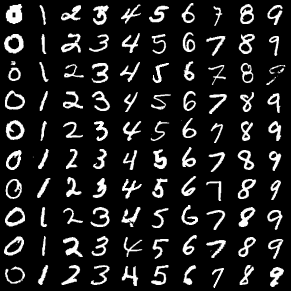
\includegraphics[scale=.9]{transfer/fig/MNIST.png}} \label{fig:single:MNIST}
		 &
		 \subfloat[USPS]{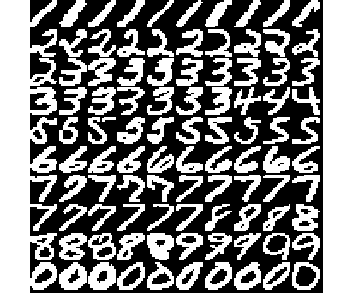
\includegraphics[scale=.9]{transfer/fig/USPS.png}}  \label{fig:single:USPS} 	
	\end{tabular}\caption{Some examples of MNIST \& USPS.}\label{fig:single:dataset}
\end{figure}

% Table generated by Excel2LaTeX from sheet 'Sheet1'
\begin{table}[htbp]\label{tab:single:MNIST}
	\centering
	\caption{Data distribution of MNIST subset}
	\begin{tabular}{|C{2cm}|C{2cm}|C{2cm}|C{2cm}|C{2cm}|C{2cm}|}
		\hline
		digit&\# examples&percentage&digit&\# examples&percentage\\\hline
		1     & 583   & 9.7\% & 6     & 511   & 8.5\% \\
		\hline
		2     & 686   & 11.4\% & 7     & 602   & 10.0\% \\\hline
		3     & 590   & 9.8\% & 8     & 609   & 10.2\% \\\hline
		4     & 652   & 10.9\% & 9     & 607   & 10.1\% \\\hline
		5     & 564   & 9.4\% & 10    & 596   & 9.9\% \\
		\hline
	\end{tabular}%
	\label{tab:addlabel}%
\end{table}%




\subsubsection{USPS}
We also use another handwritten digital dataset USPS \cite{hull1994database}. USPS contains 11,000 images and the data is evenly distributed among 10 classes, i.e. 1,100 examples for each digit. Each digit is represented as a 16x16 greyscale image.

\subsection{Experiment Setup}
In this part, we introduce the experiment set up on the two datasets. We perform experiment on different settings to simulate different scenarios for transfer learning. 

As we discussed in Section \ref{sec:single:comb}, previous work \cite{ben2010theory} show that the more similar of the source model(s) and the target task are, the more improvement the target model can get from the source model(s). When the source model and the target task are unrelated, negative transfer could happen. 
In order to test the robustness of our algorithm, we should assign the source model with different $\mathcal{D}$-relationship to the target task and test how our algorithm performs, especially when negative transfer could happen. To generate the source model(s) with different $\mathcal{D}$-relationship to the target task, we first split the dataset into 3 sub-sets: source training set, target training set and test set. Then we add the noise to the source training set and train the source model(s) from it. Therefore, as we add more noise to the source training set, the source models are more unrelated to the target task.

\begin{figure}\label{fig:single:split}
	\centering
	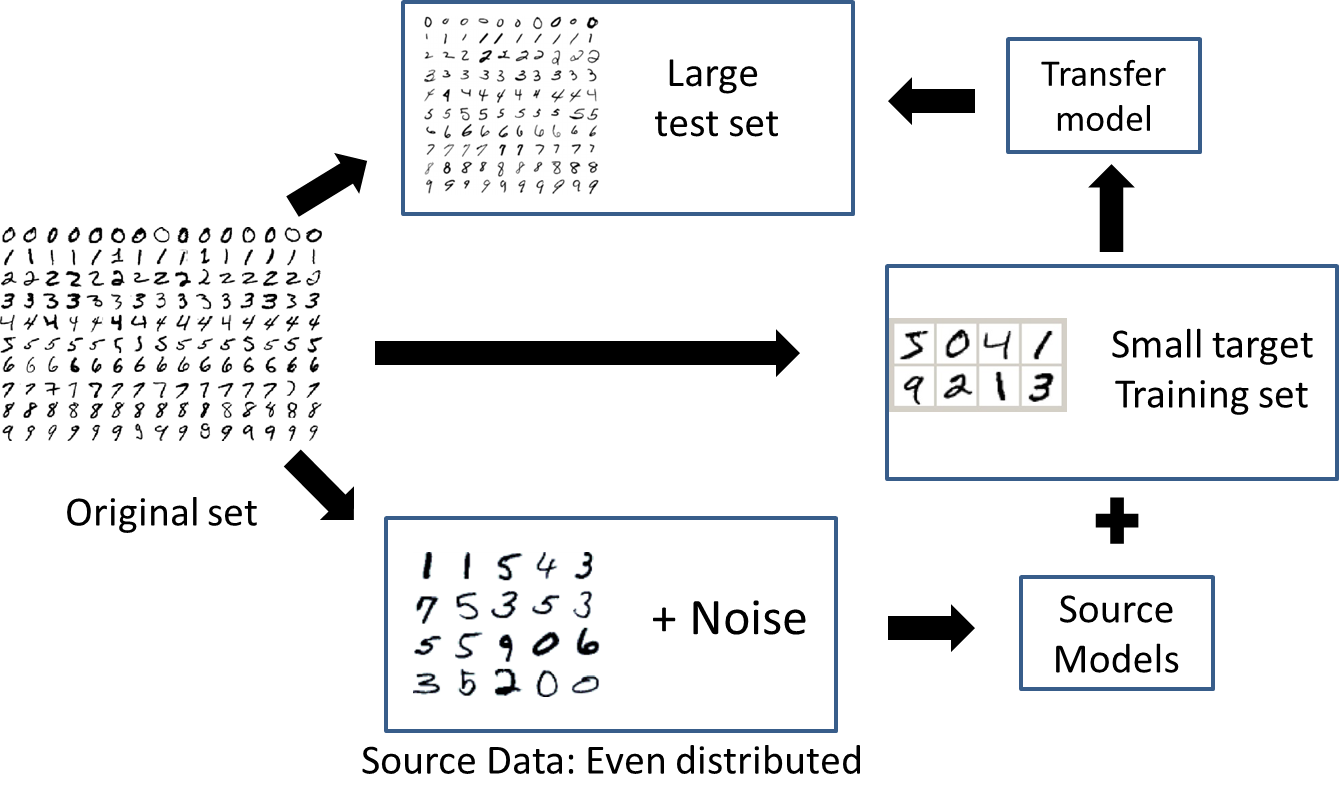
\includegraphics[scale=.7]{transfer/fig/split.png}
	\caption{Illustration of our training procedure. The data is splitted into 3 sets: a source training set, a small target training set and a large test set. Salt \& pepper noise is added into the source training set in order to generate different source models.}
\end{figure}

\begin{figure}\label{fig:single:split}
	\centering
	\subfloat[Noise Rate = 0  ]{
\includegraphics[scale=.7]{transfer/fig/0.png}}\\
	\subfloat[Noise Rate = 0.3]{
\includegraphics[scale=.7]{transfer/fig/1.png}}\\
	\subfloat[Noise Rate = 0.5]{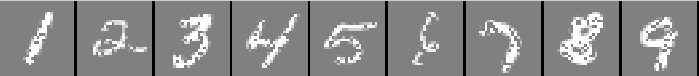
\includegraphics[scale=.7]{transfer/fig/2.png}}\\
	\subfloat[Noise Rate = 0.8]{
\includegraphics[scale=.7]{transfer/fig/3.png}}\\
	\caption{Images with different level of noise rate. By adding more slat\&pepper noise, the images become less clear.}
\end{figure}

% Table generated by Excel2LaTeX from sheet 'Sheet1'
\begin{table}[htbp]
	\centering
	\caption{Setups for our experiment on two datasets}
	\begin{tabular}{|C{5cm}|C{3cm}|C{3cm}|}
		\hline
		& MNIST & USPS \\
		\hline
		noise rate & \multicolumn{2}{c|}{0,0.2,0.3,0.5,0.8,0.9} \\\hline
		source training set size & \multicolumn{2}{c|}{100} \\\hline
		target training set size & \multicolumn{2}{c|}{5,10,15,20,25} \\\hline
		test set size & 4700  & 9700 \\
		\hline
	\end{tabular}%
	\label{tab:addlabel}%
\end{table}%
